\documentclass[14pt]{extreport}
\usepackage{fontspec}
\usepackage{polyglossia}
\usepackage{graphicx}
\setmainlanguage{russian}
\setotherlanguages{english}
\setmainfont{Times New Roman}

\setmainfont[
    Path=./fonts/,
    Extension=.ttf,
    Ligatures=TeX,
    UprightFont={*-Regular},
    BoldFont={*-Bold},
    ItalicFont={*-Italic},
    BoldItalicFont={*-BoldItalic}
    ]{BookmanOldStyle}

\newfontfamily\cyrillicfont{Times New Roman}

\usepackage[a4paper,left=30mm,right=10mm,top=20mm,bottom=20mm]{geometry}

\setlength{\parindent}{1.25cm}

\setlength{\parskip}{0pt}

\linespread{1.5}



\begin{document}
    
    \title{Реферат на тему: \\[0.5cm] \textbf{Топ 4 крутых столбов}}
    \author{Студент: Петелин Иван Андреевич \\ Группа: 2}
    \date{18.09.2024}
    
    \maketitle
    
    \chapter{Введение}
    Столбы это на самом деле очень круто, никто не задумывался но они окружают нас повсюду и стоит окинуть их взглядом снизу вверх. Это топ столбов.
    \chapter{Топ столбов}
    \section{ТОП-4 Электрический столб}
        Дефолтный стол каких миллионы, ничем не пригляден, держит провода, скука одним словом, поэтому топ 4
    \begin{figure}[h]
                \centering
                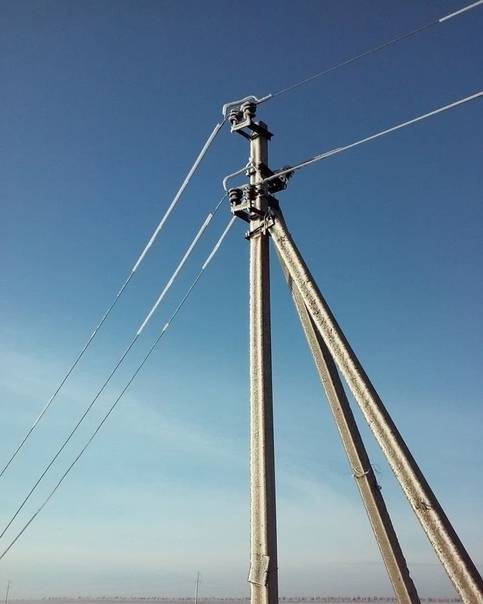
\includegraphics[width=0.5\textwidth]{elctro.jpg}
                \caption{Электростолб}
                \label{fig:example1}
            \end{figure}
            
    \section{ТОП-3 Каменный столб}
    Вот такая штука, вот это да. Я даже сам не знаю его сделали люди или природа, это больая загадка на самом деле. За такую таинственность присуждается третье место
        \begin{figure}[h]
                \centering
                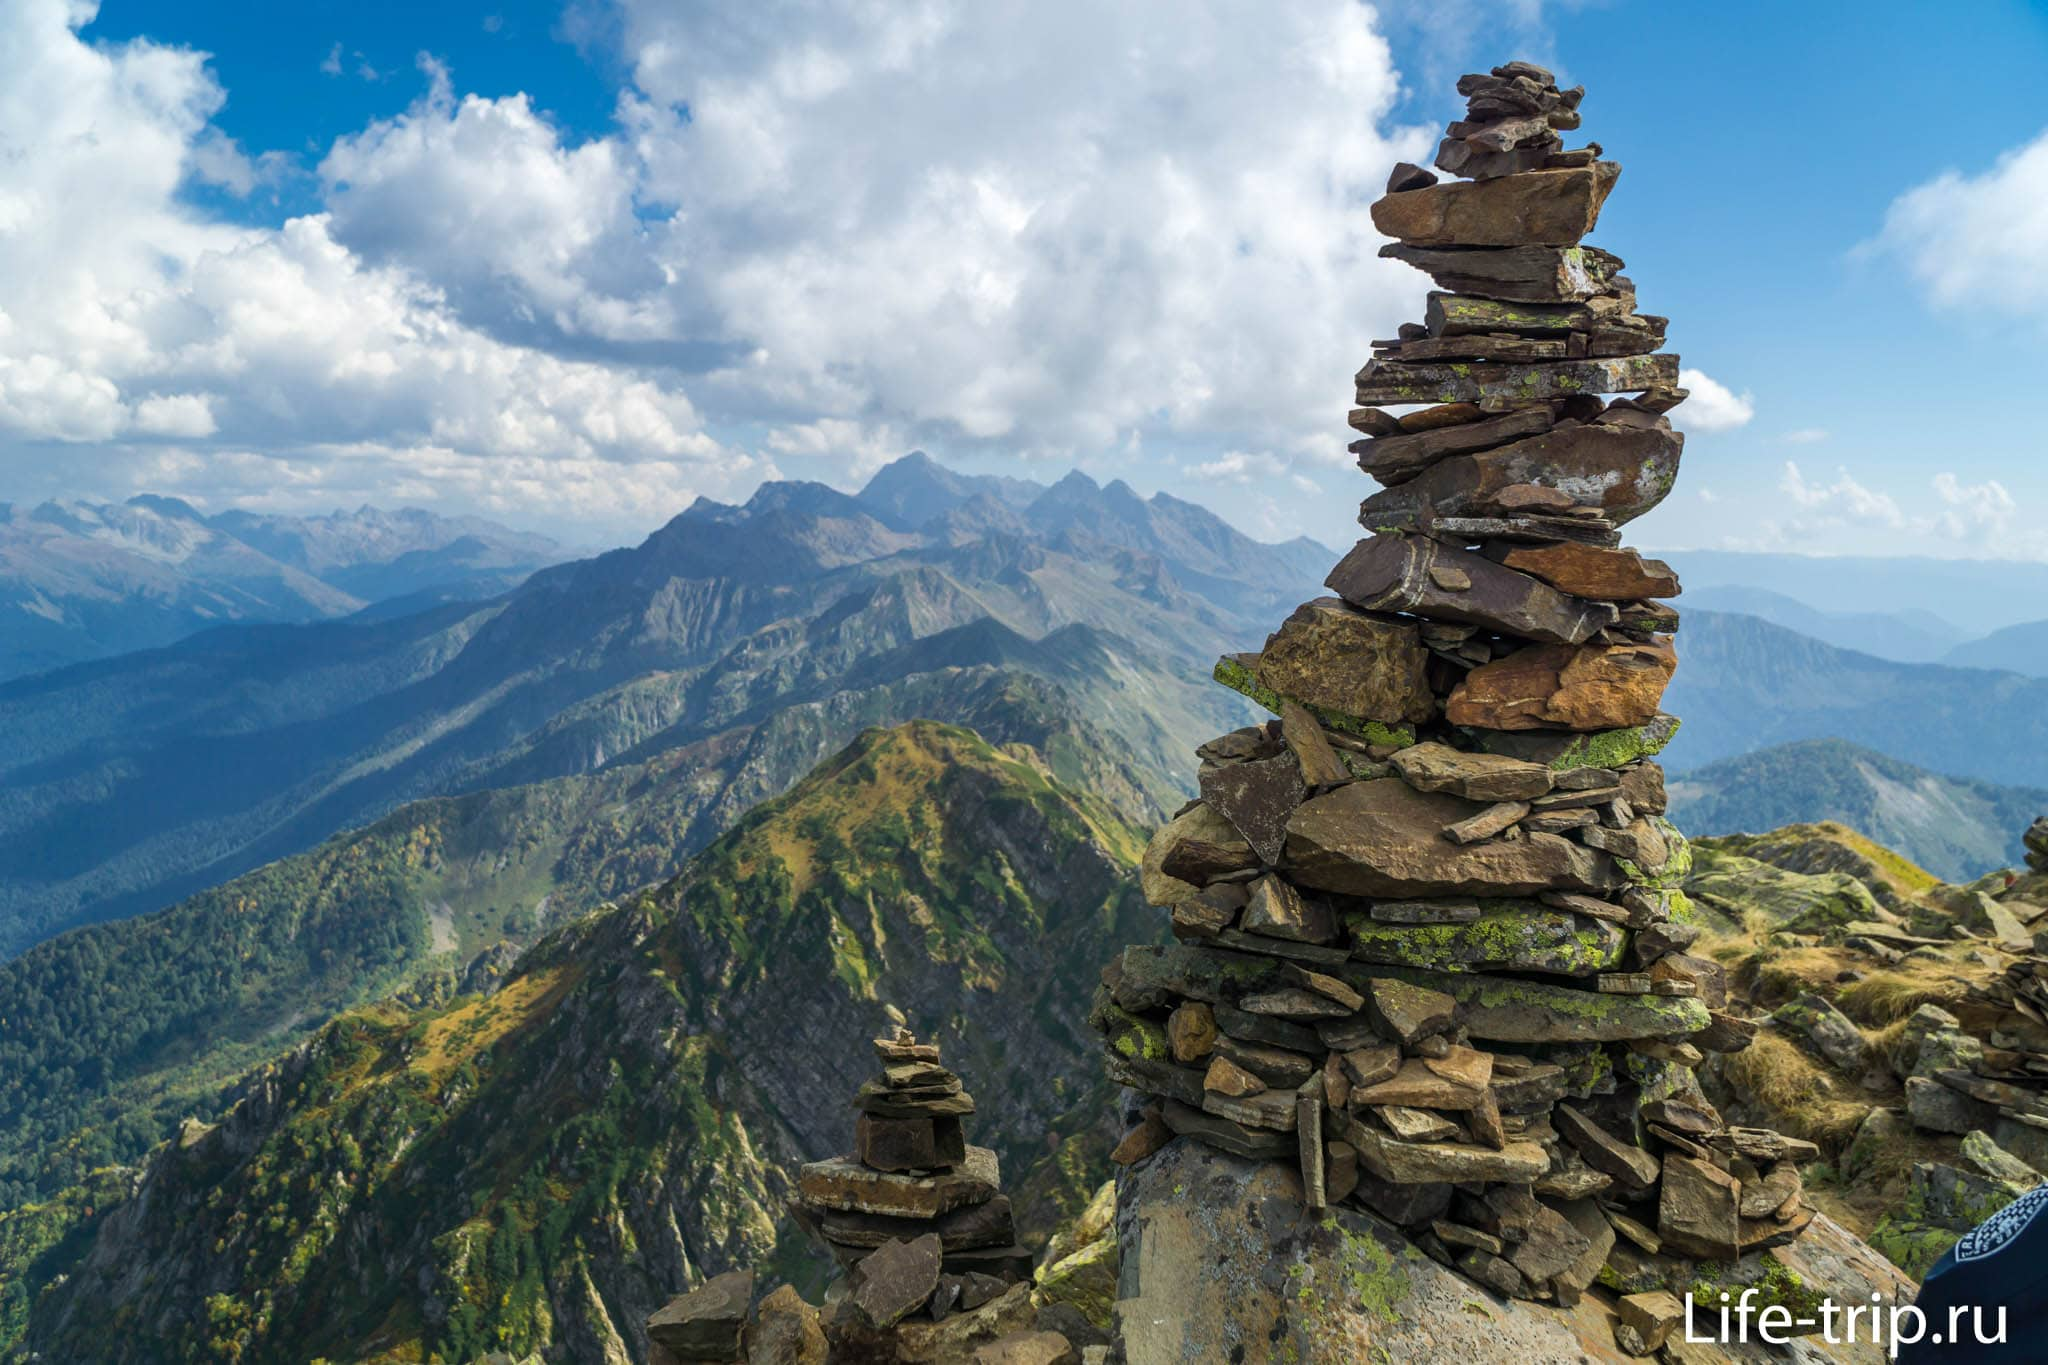
\includegraphics[width=0.5\textwidth]{kamenny.jpg}
                \caption{А какой фон, красота!}
                \label{fig:example1}
            \end{figure}
            
    \section{ТОП-2 Фонарный столб}
    Вот это да! Многие меня спросят, а почему обычный фонарный столб это топ-2 всех столбов, чем он лучше электрического столба или каменного (рис. \ref{fig:example1} ) ? А вот и расскажу!
                \begin{figure}[h]
                        \centering
                        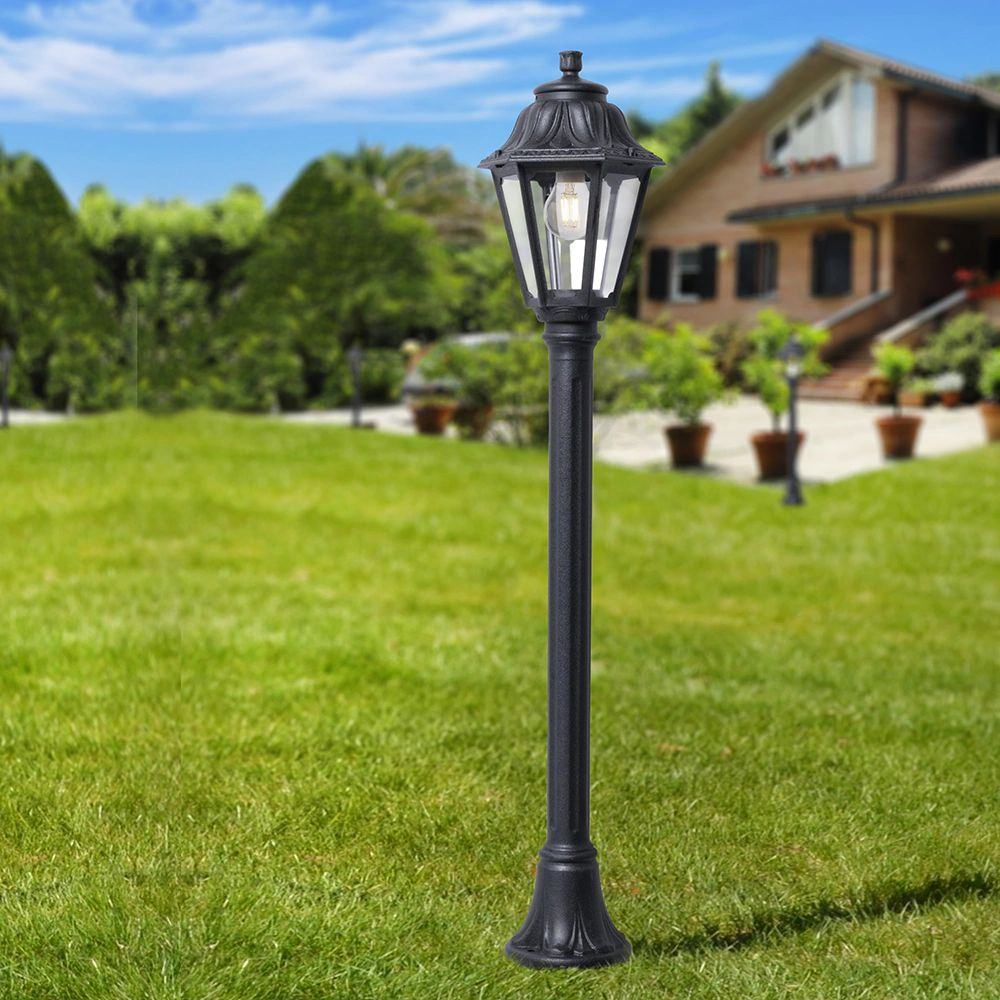
\includegraphics[width=0.5\textwidth]{stolbic.jpg}
                        \caption{В искусственной среде обитания}
                        \label{fan}
                    \end{figure}
    \subsection{Ответ}
    Фонарный столб такой куртой потому что он дает свет и еще у него красивые металические штуки!
    
    \section{ТОП-1 Огненный столб!}
    Не удивляйтесь, огненный столб реально топ-1 моего рейтинга ведь этот столб мощнее и ярче всех других, а еще может обжечь (осторожнее)!

        \begin{figure}[h]
                \centering
                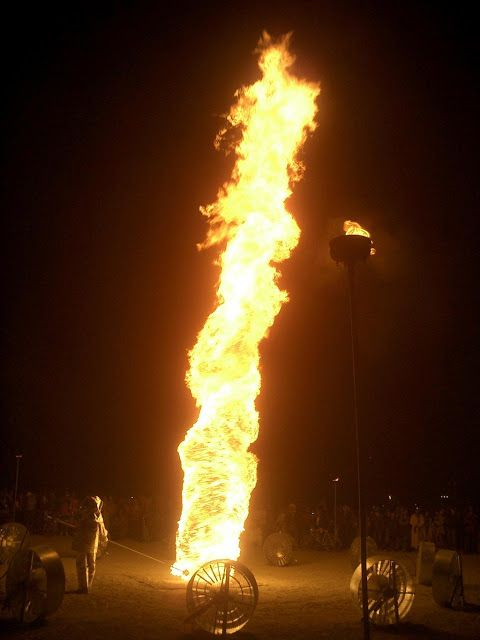
\includegraphics[width=0.5\textwidth]{ognenny.jpg}
                \caption{маленький, но жгучий!}
                \label{og}
            \end{figure}
    
    Еще одна причина что именно такой столб предстал перед врагами Моисея, это и есть ангел \textbf{Господень}, свят! свят! аминь!
    
    \chapter{Заключение}
    Итак в заверение подведем инфографику в виде \textit{столбчатой} таблицы
    \begin{table}[h]
            \centering
            \begin{tabular}{|c|c|c|с|}
                \hline
                ТОП-4 & ТОП-2 & ТОП-3 & ТОП-1 \\
                \hline
                Электрический & Каменный & Фонарный & Огненный \\
                \hline
            \end{tabular}
            \caption{ТОП}
            \label{tab:example}
        \end{table}
    \tableofcontents
    
    \section{Список литературы}
    \begin{enumerate}
    \item Яворский А.Л., Соболев А.Н. "Столбы".
    \end{enumerate}
    
\end{document}